% ============================================================================
% SmartTimeAwareStationRepair Operator — Illustration
% ============================================================================
% Compile with: pdflatex or xelatex
% Required packages: tikz, amsmath, amssymb
% ============================================================================

\documentclass[border=10pt,tikz]{standalone}
\usepackage[utf8]{inputenc}
\usepackage{amsmath,amssymb}
\usepackage{tikz}
\usetikzlibrary{arrows.meta, positioning, decorations.pathmorphing,
                calc, backgrounds, fit, shapes.geometric,
                patterns, fadings, decorations.markings}

% ── Color Palette ──
\definecolor{depot}{HTML}{2C3E50}
\definecolor{customer}{HTML}{E67E22}
\definecolor{custInsert}{HTML}{E74C3C}
\definecolor{station}{HTML}{3498DB}
\definecolor{stChosen}{HTML}{27AE60}
\definecolor{routeLine}{HTML}{7F8C8D}
\definecolor{searchZone}{HTML}{9B59B6}
\definecolor{freeCharge}{HTML}{2ECC71}
\definecolor{phase1}{HTML}{2980B9}
\definecolor{phase2a}{HTML}{8E44AD}
\definecolor{phase2b}{HTML}{D35400}
\definecolor{annotColor}{HTML}{6C3483}
\definecolor{bgGray}{HTML}{F8F9FA}
\definecolor{battLow}{HTML}{E74C3C}
\definecolor{battMed}{HTML}{F39C12}
\definecolor{battHigh}{HTML}{27AE60}
\definecolor{slackGreen}{HTML}{D5F5E3}

\begin{document}
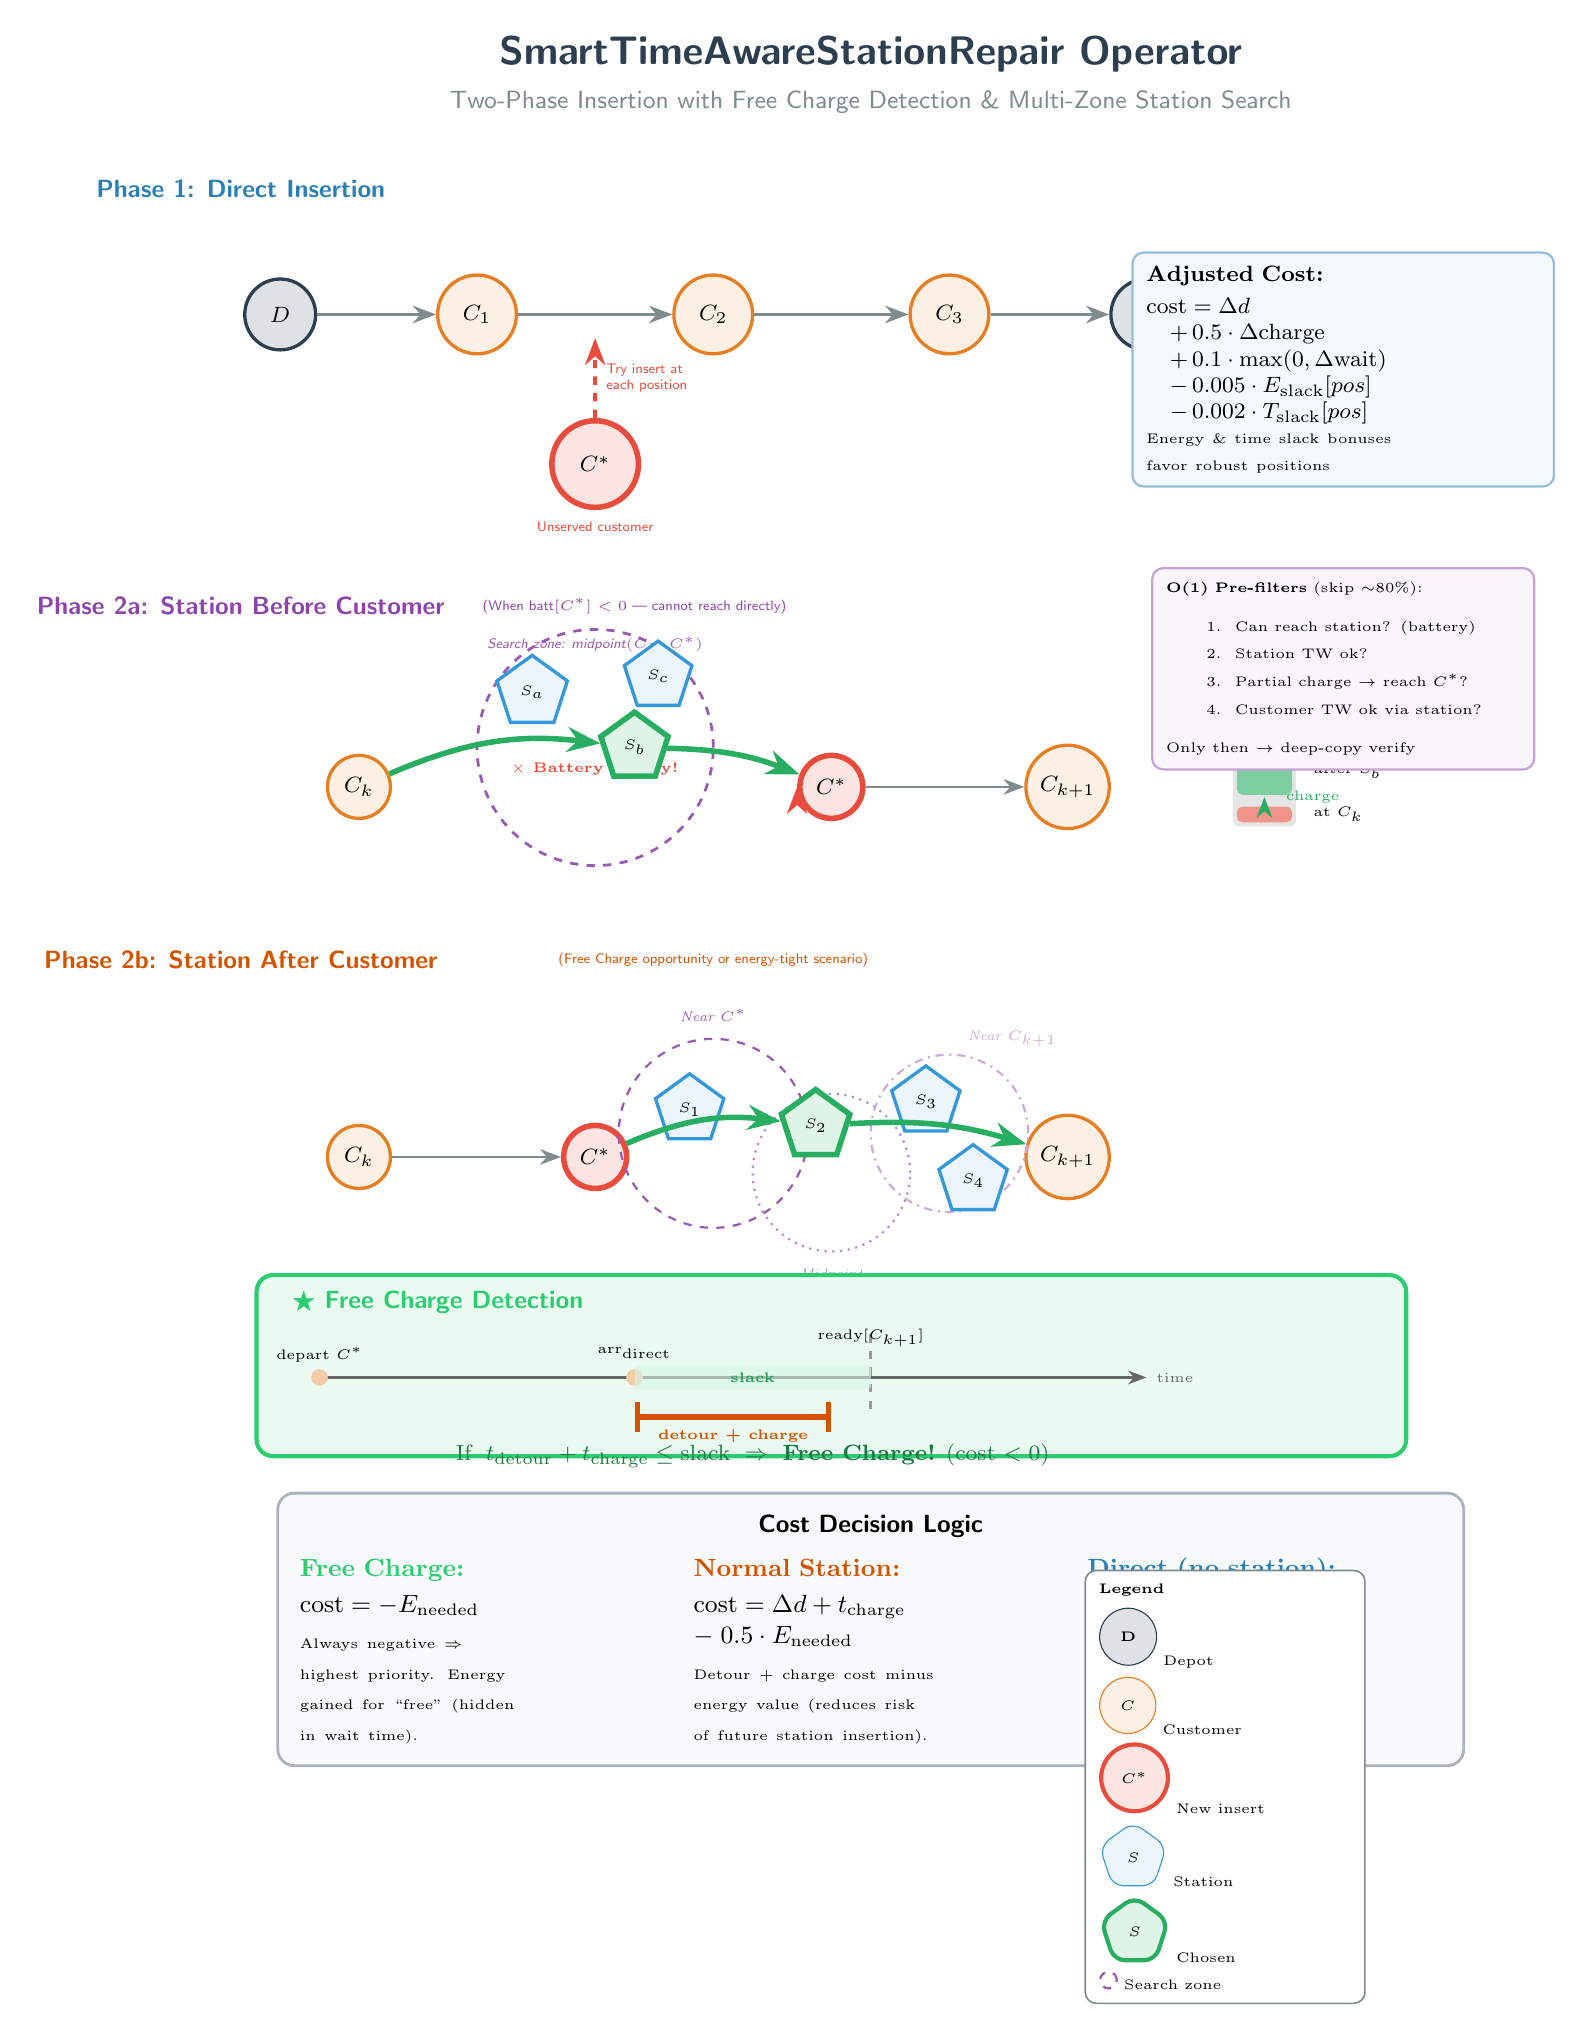
\begin{tikzpicture}[
    >=Stealth,
    every node/.style={font=\small},
    depot node/.style={
        circle, draw=depot, fill=depot!15, line width=1.2pt,
        minimum size=9mm, font=\footnotesize\bfseries
    },
    cust node/.style={
        circle, draw=customer, fill=customer!12, line width=1.2pt,
        minimum size=10mm, font=\footnotesize\bfseries
    },
    new cust/.style={
        circle, draw=custInsert, fill=custInsert!15, line width=2pt,
        minimum size=11mm, font=\footnotesize\bfseries
    },
    station node/.style={
        regular polygon, regular polygon sides=5,
        draw=station, fill=station!10, line width=1.2pt,
        minimum size=10mm, font=\footnotesize\bfseries
    },
    chosen station/.style={
        regular polygon, regular polygon sides=5,
        draw=stChosen, fill=stChosen!15, line width=2pt,
        minimum size=11mm, font=\footnotesize\bfseries
    },
    phase label/.style={
        font=\small\bfseries\sffamily, text=#1
    },
    info box/.style={
        draw=#1!50, fill=#1!5, rounded corners=4pt,
        line width=0.8pt, inner sep=5pt, font=\footnotesize
    },
    search circle/.style={
        draw=#1, fill=#1!5, line width=1pt, dashed, circle
    },
]

% ════════════════════════════════════════════════════════════════════
% TITLE
% ════════════════════════════════════════════════════════════════════
\node[font=\Large\bfseries\sffamily, text=depot] at (7.5, 12.5)
    {SmartTimeAwareStationRepair Operator};
\node[font=\small\sffamily, text=routeLine] at (7.5, 11.9)
    {Two-Phase Insertion with Free Charge Detection \& Multi-Zone Station Search};

% ════════════════════════════════════════════════════════════════════
% PART A: PHASE 1 — Direct Insertion (Without Station)
% ════════════════════════════════════════════════════════════════════

\node[phase label=phase1] at (-0.5, 10.8) {Phase 1: Direct Insertion};

% Original route
\node[depot node] (d0) at (0, 9.2) {$D$};
\node[cust node] (c1) at (2.5, 9.2) {$C_1$};
\node[cust node] (c2) at (5.5, 9.2) {$C_2$};
\node[cust node] (c3) at (8.5, 9.2) {$C_3$};
\node[depot node] (d1) at (11, 9.2) {$D$};

\foreach \a/\b in {d0/c1, c1/c2, c2/c3, c3/d1} {
    \draw[->, routeLine, line width=1.2pt] (\a) -- (\b);
}

% New customer to insert
\node[new cust] (cnew) at (4, 7.3) {$C^*$};
\node[font=\tiny\sffamily, text=custInsert] at (4, 6.5) {Unserved customer};

% Try insertion arrow
\draw[->, custInsert, line width=1.5pt, dashed]
    (cnew) -- ($(c1)!0.5!(c2) + (0,-0.3)$)
    node[midway, right, font=\tiny\sffamily, text=custInsert, text width=2.5cm, align=left]
    {Try insert at\\each position};

% Cost formula for Phase 1
\node[info box=phase1, text width=5cm, align=left] at (13.5, 8.5) {
    \textbf{Adjusted Cost:}\\[2pt]
    $\text{cost} = \Delta d$\\
    $\quad + \,0.5 \cdot \Delta\text{charge}$\\
    $\quad + \,0.1 \cdot \max(0, \Delta\text{wait})$\\
    $\quad - \,0.005 \cdot E_{\text{slack}}[pos]$\\
    $\quad - \,0.002 \cdot T_{\text{slack}}[pos]$\\[3pt]
    {\tiny Energy \& time slack bonuses\\
    favor robust positions}
};

% ════════════════════════════════════════════════════════════════════
% PART B: PHASE 2a — Station BEFORE Customer (Battery Critical)
% ════════════════════════════════════════════════════════════════════

\node[phase label=phase2a] at (-0.5, 5.5) {Phase 2a: Station Before Customer};
\node[font=\tiny\sffamily, text=phase2a] at (4.5, 5.5) 
    {(When $\text{batt}[C^*] < 0$ — cannot reach directly)};

\begin{scope}[shift={(0, 3.2)}]
    % Route segment
    \node[cust node, minimum size=8mm] (pa_prev) at (1, 0) {$C_k$};
    \node[new cust, minimum size=8mm] (pa_cust) at (7, 0) {$C^*$};
    \node[cust node, minimum size=8mm] (pa_next) at (10, 0) {$C_{k+1}$};

    % Dashed line showing impossible direct reach
    \draw[->, battLow, line width=1.5pt, densely dashed,
          decorate, decoration={markings,
          mark=at position 0.5 with {\node[above, font=\tiny\bfseries, text=battLow]
          {$\times$ Battery Empty!};}}]
        (pa_prev) -- (pa_cust);

    % Station candidates near midpoint
    \node[font=\tiny\sffamily\itshape, text=searchZone] at (4, 1.8)
        {Search zone: midpoint$(C_k, C^*)$};
    \draw[searchZone, line width=1pt, dashed] (4, 0.5) circle (1.5cm);

    \node[station node, minimum size=7mm] (pa_s1) at (3.2, 1.2) {\tiny$S_a$};
    \node[chosen station, minimum size=7mm] (pa_s2) at (4.5, 0.5) {\tiny$S_b$};
    \node[station node, minimum size=7mm] (pa_s3) at (4.8, 1.4) {\tiny$S_c$};

    % Chosen path: prev -> station -> cust
    \draw[->, stChosen, line width=2pt]
        (pa_prev) to[bend left=15] (pa_s2);
    \draw[->, stChosen, line width=2pt]
        (pa_s2) to[bend left=10] (pa_cust);
    \draw[->, routeLine, line width=1pt]
        (pa_cust) -- (pa_next);

    % Battery gauge
    \begin{scope}[shift={(12.5, -0.5)}]
        \node[font=\tiny\sffamily\bfseries] at (0, 1.4) {Battery Level};
        % Gauge background
        \fill[black!10, rounded corners=2pt] (-0.4, 0) rectangle (0.4, 1.2);
        % Low level at prev
        \fill[battLow!60, rounded corners=2pt] (-0.35, 0.05) rectangle (0.35, 0.25);
        \node[font=\tiny, right] at (0.5, 0.15) {at $C_k$};
        % After charge
        \fill[battHigh!60, rounded corners=2pt] (-0.35, 0.4) rectangle (0.35, 1.0);
        \node[font=\tiny, right] at (0.5, 0.7) {after $S_b$};
        % Charge arrow
        \draw[->, stChosen, line width=1pt] (0, 0.28) -- (0, 0.37)
            node[right, font=\tiny, text=stChosen, xshift=4pt] {charge};
    \end{scope}

    % O(1) pre-filter annotation
    \node[info box=phase2a, text width=4.5cm, align=left, font=\tiny] at (13.5, 1.5) {
        \textbf{O(1) Pre-filters} (skip $\sim$80\%):
        \begin{enumerate}\setlength{\itemsep}{0pt}
            \item Can reach station? (battery)
            \item Station TW ok?
            \item Partial charge $\to$ reach $C^*$?
            \item Customer TW ok via station?
        \end{enumerate}
        Only then $\to$ deep-copy verify
    };
\end{scope}

% ════════════════════════════════════════════════════════════════════
% PART C: PHASE 2b — Station AFTER Customer (Free Charge / Proactive)
% ════════════════════════════════════════════════════════════════════

\node[phase label=phase2b] at (-0.5, 1.0) {Phase 2b: Station After Customer};
\node[font=\tiny\sffamily, text=phase2b] at (5.5, 1.0) 
    {(Free Charge opportunity or energy-tight scenario)};

\begin{scope}[shift={(0, -1.5)}]
    % Route segment
    \node[cust node, minimum size=8mm] (pb_prev) at (1, 0) {$C_k$};
    \node[new cust, minimum size=8mm] (pb_cust) at (4, 0) {$C^*$};
    \node[cust node, minimum size=8mm] (pb_next) at (10, 0) {$C_{k+1}$};

    % Three search zones
    % Zone 1: Near customer
    \draw[searchZone, line width=0.8pt, dashed] (5.5, 0.3) circle (1.2cm);
    \node[font=\tiny\itshape, text=searchZone] at (5.5, 1.8) {Near $C^*$};

    % Zone 2: Midpoint
    \draw[searchZone!70, line width=0.8pt, dotted] (7, -0.2) circle (1.0cm);
    \node[font=\tiny\itshape, text=searchZone!70] at (7, -1.5) {Midpoint};

    % Zone 3: Near next
    \draw[searchZone!50, line width=0.8pt, dash dot] (8.5, 0.3) circle (1.0cm);
    \node[font=\tiny\itshape, text=searchZone!50] at (9.3, 1.5) {Near $C_{k+1}$};

    % Station candidates
    \node[station node, minimum size=6mm] (pb_s1) at (5.2, 0.6) {\tiny$S_1$};
    \node[chosen station, minimum size=7mm] (pb_s2) at (6.8, 0.4) {\tiny$S_2$};
    \node[station node, minimum size=6mm] (pb_s3) at (8.2, 0.7) {\tiny$S_3$};
    \node[station node, minimum size=6mm] (pb_s4) at (8.8, -0.3) {\tiny$S_4$};

    % Chosen path
    \draw[->, routeLine, line width=1pt] (pb_prev) -- (pb_cust);
    \draw[->, stChosen, line width=2pt] (pb_cust) to[bend left=15] (pb_s2);
    \draw[->, stChosen, line width=2pt] (pb_s2) to[bend left=10] (pb_next);

    % ── FREE CHARGE DETECTION ──
    \begin{scope}[shift={(0, -2.5)}]
        \fill[freeCharge!10, rounded corners=6pt]
            (-0.3, -1.3) rectangle (14.3, 1.0);
        \draw[freeCharge, line width=1.5pt, rounded corners=6pt]
            (-0.3, -1.3) rectangle (14.3, 1.0);

        \node[font=\small\bfseries\sffamily, text=freeCharge] at (2, 0.65)
            {$\bigstar$ Free Charge Detection};

        % Timeline visualization
        \begin{scope}[shift={(0.5, -0.3)}]
            % Time axis
            \draw[->, black!60, line width=0.8pt] (0, 0) -- (10.5, 0)
                node[right, font=\tiny] {time};

            % Direct arrival
            \fill[customer!40] (0, 0) circle (3pt);
            \node[font=\tiny, above=2pt] at (0, 0) {depart $C^*$};

            \fill[customer!40] (4, 0) circle (3pt);
            \node[font=\tiny, above=2pt] at (4, 0.05) {arr$_\text{direct}$};

            % Ready time of next
            \draw[black!40, line width=1pt, dashed] (7, -0.4) -- (7, 0.6);
            \node[font=\tiny, above=2pt] at (7, 0.2) {ready$[C_{k+1}]$};

            % Slack = waiting time
            \fill[slackGreen, opacity=0.6, rounded corners=1pt]
                (4, -0.15) rectangle (7, 0.15);
            \node[font=\tiny\bfseries, text=freeCharge!80!black] at (5.5, 0) {slack};

            % Detour + charge time
            \draw[phase2b, line width=2pt, |-|] (4, -0.5) -- (6.5, -0.5);
            \node[font=\tiny\bfseries, text=phase2b, below=1pt] at (5.25, -0.5)
                {detour + charge};

            % Condition
            \node[font=\footnotesize, text=freeCharge!60!black] at (5.5, -1.0)
                {If \;$t_\text{detour} + t_\text{charge} \leq \text{slack}$
                 \;$\Rightarrow$\; \textbf{Free Charge!} (cost $< 0$)};
        \end{scope}
    \end{scope}
\end{scope}

% ════════════════════════════════════════════════════════════════════
% PART D: COST DECISION LOGIC (Bottom)
% ════════════════════════════════════════════════════════════════════

\begin{scope}[shift={(0, -7.5)}]
    \node[draw=depot!40, fill=bgGray, rounded corners=6pt, line width=1pt,
          inner sep=8pt, text width=14.5cm, align=left] at (7.5, 0) {
        \begin{minipage}{\textwidth}
        \centering
        {\bfseries\sffamily Cost Decision Logic}
        \end{minipage}

        \vspace{5pt}
        \begin{minipage}[t]{4.5cm}
            \textbf{\color{freeCharge} Free Charge:}\\[2pt]
            $\text{cost} = -E_\text{needed}$\\[2pt]
            {\tiny Always negative $\Rightarrow$\\
            highest priority. Energy\\
            gained for ``free'' (hidden\\
            in wait time).}
        \end{minipage}
        \hfill
        \begin{minipage}[t]{4.5cm}
            \textbf{\color{phase2b} Normal Station:}\\[2pt]
            $\text{cost} = \Delta d + t_\text{charge}$\\
            $\quad\quad\; - \;0.5 \cdot E_\text{needed}$\\[2pt]
            {\tiny Detour + charge cost minus\\
            energy value (reduces risk\\
            of future station insertion).}
        \end{minipage}
        \hfill
        \begin{minipage}[t]{4.5cm}
            \textbf{\color{phase1} Direct (no station):}\\[2pt]
            $\text{cost} = \Delta d + 0.5\Delta q$\\
            $\quad + \;0.1\,\Delta w - \text{bonuses}$\\[2pt]
            {\tiny Standard insertion cost\\
            with energy \& time slack\\
            tiebreakers for robustness.}
        \end{minipage}
    };
\end{scope}

% ════════════════════════════════════════════════════════════════════
% LEGEND (Bottom Right)
% ════════════════════════════════════════════════════════════════════

\begin{scope}[shift={(12, -9.5)}]
    \node[draw=routeLine, fill=white, rounded corners=4pt, line width=0.6pt,
          inner sep=5pt, text width=3.2cm, align=left, font=\tiny] (legend) at (0,0) {
        \textbf{Legend}\\[3pt]
        \tikz\node[circle, draw=depot, fill=depot!15, minimum size=4mm, font=\tiny\bfseries]{D}; Depot\\[2pt]
        \tikz\node[circle, draw=customer, fill=customer!12, minimum size=4mm, font=\tiny]{$C$}; Customer\\[2pt]
        \tikz\node[circle, draw=custInsert, fill=custInsert!15, minimum size=4mm, line width=1.5pt, font=\tiny]{$C^*$}; New insert\\[2pt]
        \tikz\node[regular polygon, regular polygon sides=5, draw=station, fill=station!10, minimum size=4mm, font=\tiny]{$S$}; Station\\[2pt]
        \tikz\node[regular polygon, regular polygon sides=5, draw=stChosen, fill=stChosen!15, minimum size=4mm, line width=1.5pt, font=\tiny]{$S$}; Chosen\\[2pt]
        \tikz\draw[searchZone, dashed, line width=0.8pt] (0,0) circle (3pt); Search zone
    };
\end{scope}

\end{tikzpicture}
\end{document}
